Machine Learning (ML) is a method of training models using sets of data to recognise patterns so that a trained model is capable of making predictions or decisions without explicitly being told what to do.\\ \\
The three main categories of ML are:
\begin{enumerate}
    \item Supervised Learning: the model is give the training data and a set of labels for what each piece of datum is. It is meant to learn from these data-label combos.
    
    \item Unsupervised Learning: the model has no labels and instead tries to find hidden patterns in the data.
    
    \item Reinforcement Learning: the agent tries to reach a certain goal and is given a score/reward depending on how well it achieves its goal.
\end{enumerate}
For the purposes of this project, we will only be focusing on Supervised Learning algorithms. For unsupervised learning it would become much more difficult to properly evaluate if the model is being tampered with. Human intervention is needed to check what hidden patterns the model is finding, which is not sustainable in this case.


\subsection{Neural Networks}
A Neural Network (NN) is a form of ML in which the ML model learns from its experiences with a given set of data. It achieves this through assigning weights to the connections between ``nodes" (like artificial neurons \cite{neurons}) in the network of the model. For models beyond 1 layer in depth, we also have the use of back-propagation (finding the gradient of the loss with respect to each of the weights) which makes it possible to apply efficient gradient descent for finding the optimal point. This is because these ML problems are often evaluated with a loss function where the purpose is to minimise the loss. A common loss function is Mean Squared Error (MSE) which minimises the average of squared difference between predictions and actual observations:
\begin{equation}
    MSE = \dfrac{1}{n} \Sigma (\hat{y} - y_i)^2
\end{equation}
An example of a basic NN is shown below where the thickness of each line represents the relative size of the weights for each connection.
\begin{figure}[htbp]
	\centering
    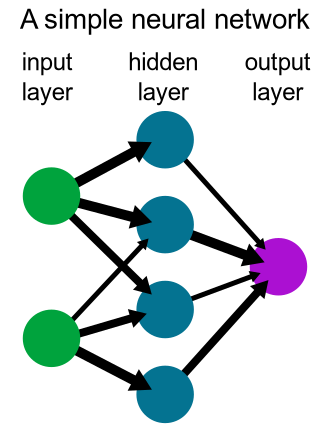
\includegraphics[scale=0.3]{background/neural_network.png}
	\caption{Neural Network image from Wikipedia, the free Encyclopedia}
	\label{fig:nn}
\end{figure}

\subsection{Deep Learning}
Deep Learning (DL) is a subset of Machine Learning that focuses on NNs with many layers. A conventional NN would only have 1 hidden layer whereas a DL network could go into the 10s or 100s (or more!). This is to accommodate ever-increasing dataset sizes. In the modern age, the sheer increase in data and parameters associated with ML is getting so large that certain problems require DL networks to solve them. This is so that every minute feature and detail can be extracted from the datasets and be properly represented by the model \cite{deeplearningbook}.\\ \\
They also include the use of activation functions between the layers. An activation function creates an output based on the output of the previous layer by applying a non-linear function to change it. Some of the most common to use are the $\tanh$ function and Rectified Linear Unit (ReLU \cite{relu}). We show some examples in \ref{tbl:activation-tbl}. \\ \\
For constructing DL models we will need to use some combination of these activation functions (and potentially others not mentioned \cite{wiki:activation}).

\newcommand{\tanhFunc}{
    $\tanh(x) = \dfrac{e^x - e^{-x}}{e^x + e^{-x}}$
}
\newcommand{\ReluFunc}{
    $ReLU(x) =
    \begin{cases}
      0 \hspace{0.5cm} $if $ x \leq 0\\    
      x \hspace{0.5cm} $if $ x > 0
    \end{cases}
    $
}
\newcommand{\SigmoidFunc}{
    $\sigma(x) = \dfrac{1}{1 + e^{-x}}$
}

\newcommand{\tanhDerivative}{
    $1 - \tanh(x)^2$
}
\newcommand{\ReluDerivative}{
    $
    \begin{cases}
      0 \hspace{0.5cm} $if $ x < 0\\
      1 \hspace{0.5cm} $if $ x > 0\\
      undefined \hspace{0.5cm} $if $ x == 0
    \end{cases}
    $
}
\newcommand{\SigmoidDerivative}{
    $\sigma(x)(1 - \sigma(x))$
}

\pgfplotsset{width=3.3cm,compat=1.9}
\newcommand{\sigmoidGraph}{
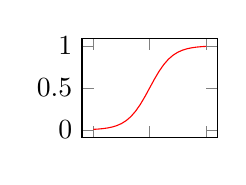
\begin{tikzpicture}
    \begin{axis}[xticklabels={,,}]
    \addplot[color=red]{1/(1 + exp(-x)};
    \end{axis}
\end{tikzpicture}
}
\newcommand{\tanhGraph}{
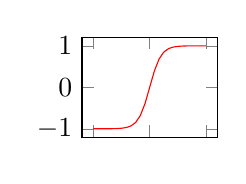
\begin{tikzpicture}
    \begin{axis}[xticklabels={,,}]
    \addplot[color=red]{(exp(x) - exp(-x))/(exp(x) + exp(-x))};
    \end{axis}
\end{tikzpicture}
}
\newcommand{\reluGraph}{
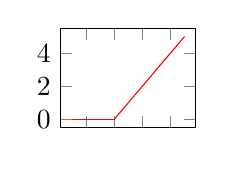
\begin{tikzpicture}
    \begin{axis}[
        domain=-3:5,
        xticklabels={,,},
        ]
        \addplot+[mark=none,red,domain=-3:0] {0};
        \addplot+[mark=none,red,domain=0:5] {x};
    \end{axis}
\end{tikzpicture}
}

\begin{center}
    \begin{longtable}{ | m{3.5em} | m{12.3em} | m{10.9em} | m{5.6em} | }
    \caption{Activation Function Table}
    \label{tbl:activation-tbl}
    \hline
    \textbf{Name} & \textbf{Function} & \textbf{Derivative} & \textbf{Example} \ \\ \hline
    tanh & \tanhFunc & \tanhDerivative & \tanhGraph \ \\ \hline
    ReLU & \ReluFunc & \ReluDerivative & \reluGraph \ \\ \hline
    Sigmoid & \SigmoidFunc & \SigmoidDerivative & \sigmoidGraph \ \\ \hline
    \end{longtable}
\end{center}

How these activation functions are used and when they are used can have an effect on the performance of a NN. Even fine-tuning certain combinations of activation functions can greatly improve performance \cite{activation_combined}.

\subsection{Convolutional Neural Networks}
DL models can be used for a variety of tasks but one that is quite common is that of image recognition. The popular structure for specific types of DL networks that focus on this is that of Convolutional Neural Networks (CNN). While typical NNs struggle in the complexity and detail of images, CNNs are more able to ``successfully capture the Spatial and Temporal dependencies in an image through the application of relevant filters" \cite{eli5_convnet}. The number of layers could in theory be increased but that adds vast computational power and it could lead to the over-fitting of the network. \\ \\
Instead we go for different architecture that consists of three distinct types of layers \cite{convnet}:
\begin{enumerate}
    \item \textbf{Convolutional Layer:} this layer takes a predefined kernel \cite{kernel} and applies it to the 2D image. If the input has more than one channel (e.g. an RGB image), then it is applied to each channel. The kernel that is used can change which features are highlighted and extracted depending on the use case. Some common kernels in Computer Vision are blurring kernels and Sobel kernels.The size of the kernel and how much it strides by in each step can decide as to how much reduction in dimensions there are.
    
    \item \textbf{Pooling Layer:} this layer is used to help decrease the spatial size of the previously convolved feature. This can then in turn decreases the processing power required to process the data as the size of the dimensions can be greatly reduced. This can be quite destructive to the data and so 2 more common approaches are to use a 2x2 kernel with a stride of 2 or to use a 3x3 kernel with a stride of two. The latter allows for overlap of the pixels but a kernel size above 3x3 can result in greatly decreased performance. Pooling is used to help detect patterns in images that are usually far too big for smaller kernels to detect actual patterns.
    
    \item \textbf{Fully-Connected Layer:} this acts like a typical NN and will try and form scores for the relevant classes/predictions based while connected in the standard way of being connected to all the neurons of the previous layer.
\end{enumerate}
An example of how these layers come together and form a CNN is below:
\begin{figure}[htbp]
	\centering
    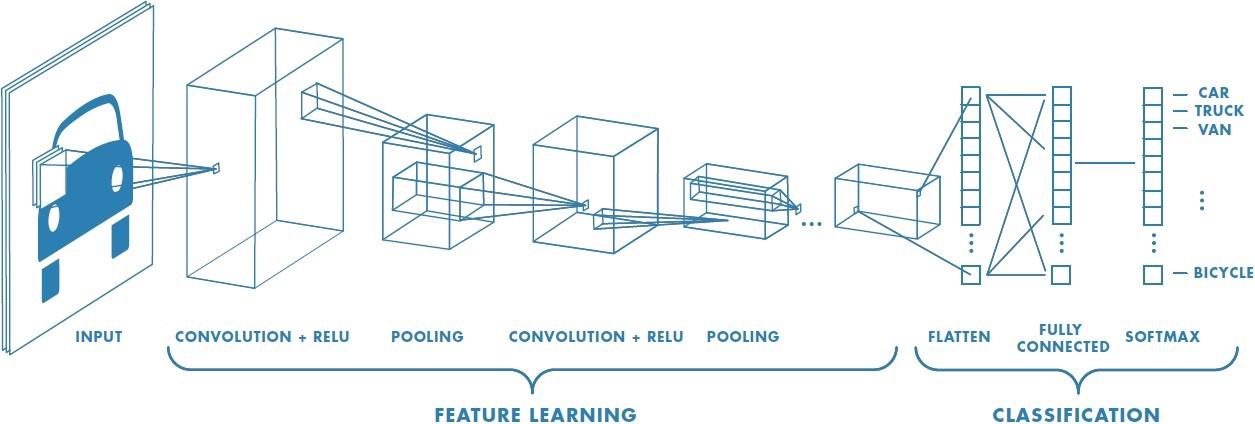
\includegraphics[scale=0.3]{background/cnn_example.jpeg}
    \caption{Visual Representation of CNN Layers \cite{eli5_convnet}}
    \label{fig:cnn-layers}
\end{figure}

For simple datasets like MNIST (where the dimensions of the images is only 28x28 and the image itself is fairly basic) we don't need a particularly complex NN beyond having the initial layer contain 784 (28x28) weights and so it doesn't necessarily benefit from a CNN. For something like the MedMNIST datasets, they are not in a higher dimension but are of higher complexity than that of standard MNIST and so more greatly benefit from the use of a CNN. Other examples of datasets that benefit this way are FashionMNIST \cite{fashion} and CIFAR-10 \cite{cifar}.\\ \\
One difference to note about the initial layer of a CNN compared to a standard NN is that it remains represented as a 2D array instead of being streamed into a 1D vector. This is something that allows the network to help recognise the patterns better as it retains the structure of the original image more precisely.
